\hypertarget{stm32f4xx__hal__dma__ex_8c}{}\section{Dokumentacja pliku S\+T\+M/\+W\+D\+S\+\_\+\+Kosc\+\_\+\+Linux/\+Drivers/\+S\+T\+M32\+F4xx\+\_\+\+H\+A\+L\+\_\+\+Driver/\+Src/stm32f4xx\+\_\+hal\+\_\+dma\+\_\+ex.c}
\label{stm32f4xx__hal__dma__ex_8c}\index{S\+T\+M/\+W\+D\+S\+\_\+\+Kosc\+\_\+\+Linux/\+Drivers/\+S\+T\+M32\+F4xx\+\_\+\+H\+A\+L\+\_\+\+Driver/\+Src/stm32f4xx\+\_\+hal\+\_\+dma\+\_\+ex.\+c@{S\+T\+M/\+W\+D\+S\+\_\+\+Kosc\+\_\+\+Linux/\+Drivers/\+S\+T\+M32\+F4xx\+\_\+\+H\+A\+L\+\_\+\+Driver/\+Src/stm32f4xx\+\_\+hal\+\_\+dma\+\_\+ex.\+c}}


D\+MA Extension H\+AL module driver This file provides firmware functions to manage the following functionalities of the D\+MA Extension peripheral\+:  


{\ttfamily \#include \char`\"{}stm32f4xx\+\_\+hal.\+h\char`\"{}}\newline
Wykres zależności załączania dla stm32f4xx\+\_\+hal\+\_\+dma\+\_\+ex.\+c\+:\nopagebreak
\begin{figure}[H]
\begin{center}
\leavevmode
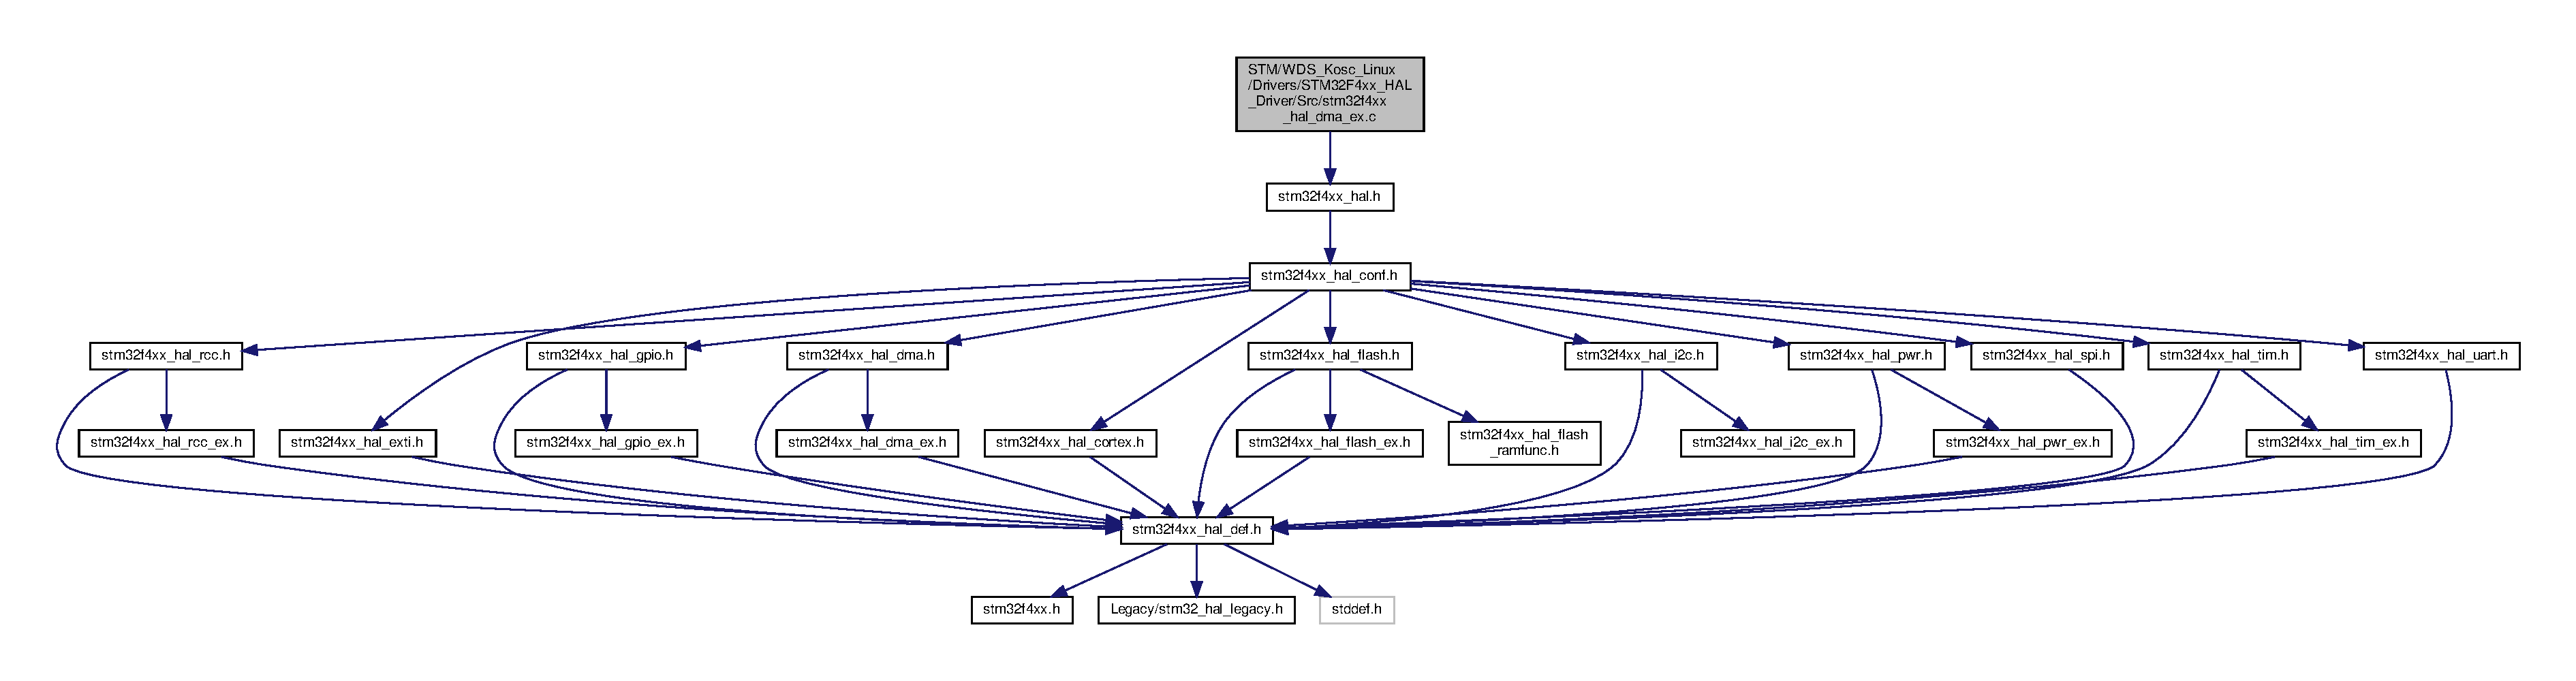
\includegraphics[width=350pt]{stm32f4xx__hal__dma__ex_8c__incl}
\end{center}
\end{figure}


\subsection{Opis szczegółowy}
D\+MA Extension H\+AL module driver This file provides firmware functions to manage the following functionalities of the D\+MA Extension peripheral\+: 

\begin{DoxyAuthor}{Autor}
M\+CD Application Team
\begin{DoxyItemize}
\item Extended features functions
\end{DoxyItemize}
\end{DoxyAuthor}
\begin{DoxyVerb}==============================================================================
                      ##### How to use this driver #####
==============================================================================
[..]
The DMA Extension HAL driver can be used as follows:
 (#) Start a multi buffer transfer using the HAL_DMA_MultiBufferStart() function
     for polling mode or HAL_DMA_MultiBufferStart_IT() for interrupt mode.
                 
   -@-  In Memory-to-Memory transfer mode, Multi (Double) Buffer mode is not allowed.
   -@-  When Multi (Double) Buffer mode is enabled the, transfer is circular by default.
   -@-  In Multi (Double) buffer mode, it is possible to update the base address for 
        the AHB memory port on the fly (DMA_SxM0AR or DMA_SxM1AR) when the stream is enabled. \end{DoxyVerb}


\begin{DoxyAttention}{Uwaga}

\end{DoxyAttention}
\subsubsection*{\begin{center}\copyright{} Copyright (c) 2017 S\+T\+Microelectronics. All rights reserved.\end{center} }

This software component is licensed by ST under B\+SD 3-\/\+Clause license, the \char`\"{}\+License\char`\"{}; You may not use this file except in compliance with the License. You may obtain a copy of the License at\+: opensource.\+org/licenses/\+B\+S\+D-\/3-\/\+Clause 